In the first section of the assignment we were asked to run our supervised classifier on the entire dataset. In figure~\ref{fig:img1} we can inspect the result of running the Random Forest model fit on the whole dataset.
A colorbar on the right side of the figure shows the class-membership probability of the data points. The colorbar ranges from -1 to 1 where -1 is class 1 and 1 is class 2. The colorbar is centered at 0, which is the unlabeled class. 
The colorbar is a good visual representation of the class-membership probability of the data points. The predictions of the model are shown in figure~\ref{fig:img2}. The predictions are shown as the background color of the plot.

\begin{figure}[H]
    \centering
    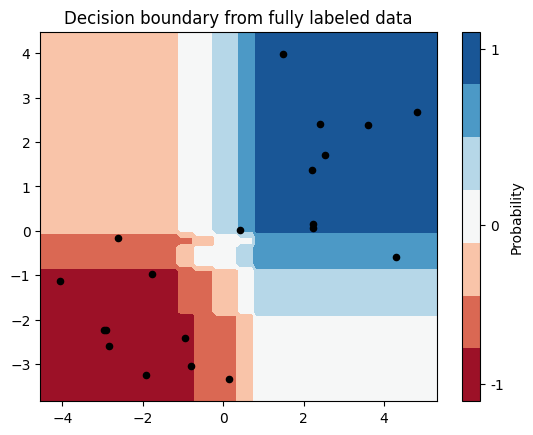
\includegraphics[width=0.5\textwidth]{images/img1.png}
    \caption{Random Forest Model Fit on the Whole Dataset}
    \label{fig:img1}
\end{figure}

\begin{figure}[H]
    \centering
    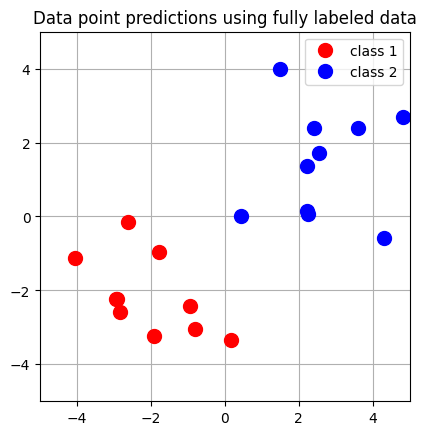
\includegraphics[width=0.5\textwidth]{images/img2.png}
    \caption{Random Forest Model Predictions}
    \label{fig:img2}
\end{figure}

In the upcoming figures, figure~\ref{fig:img3} and figure~\ref{fig:img4}, we can see the results of running the Random Forest model fit on the two-point dataset.
The colorbar on the right side of the figure shows the class-membership probability of the data points. The colorbar ranges from -1 to 1 where -1 is class 1 and 1 is class 2. The colorbar is centered at 0, which is the unlabeled class.

\begin{figure}[H]
    \centering
    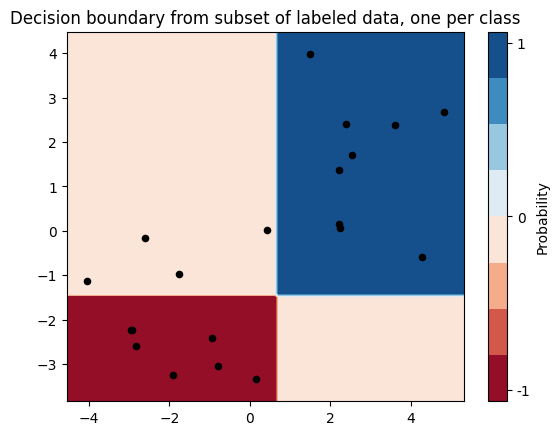
\includegraphics[width=0.5\textwidth]{images/img3.png}
    \caption{Random Forest Model Fit on the Two-Point Dataset}
    \label{fig:img3}
\end{figure}

\begin{figure}[H]
    \centering
    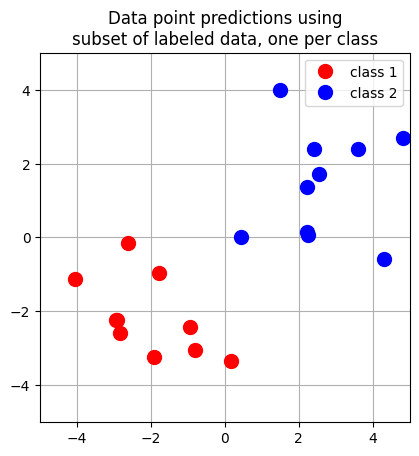
\includegraphics[width=0.5\textwidth]{images/img4.png}
    \caption{Random Forest Model Predictions}
    \label{fig:img4}
\end{figure}

The graphs of the predictions shown in figure~\ref{fig:img2} and figure~\ref{fig:img4} are similar. The predictions are shown as the background color of the plot. 

As described in the methodology section, the wrapper method for semi-supervised learning was implemented using the random forest classifier. The per-iteration results of this method are shown in figure~\ref{fig:img5} through figure~\ref{fig:img12}.  

\begin{figure}[H]
    \centering
    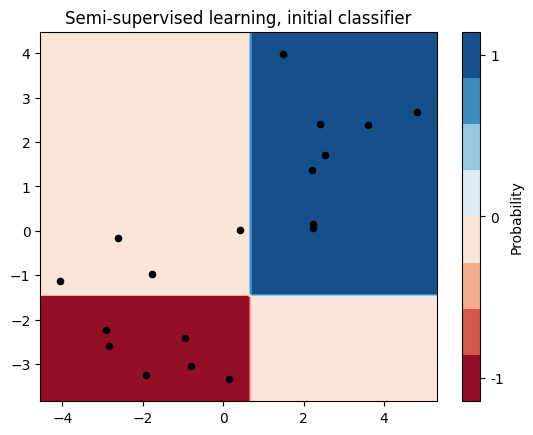
\includegraphics[width=0.5\textwidth]{images/img5.png}
    \caption{Wrapper Method Iteration 1}
    \label{fig:img5}
\end{figure}

\begin{figure}[H]
    \centering
    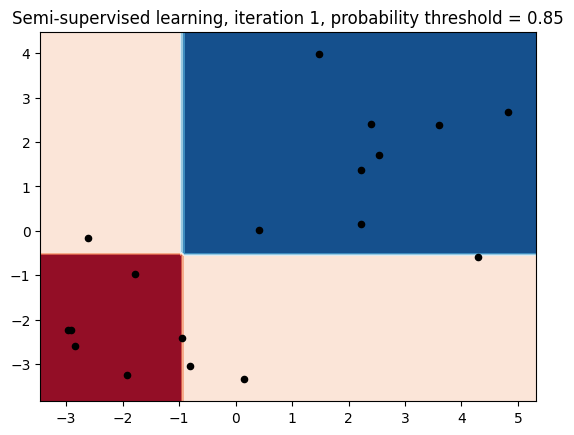
\includegraphics[width=0.5\textwidth]{images/img6.png}
    \caption{Wrapper Method Iteration 2}
    \label{fig:img6}
\end{figure}

\begin{figure}[H]
    \centering
    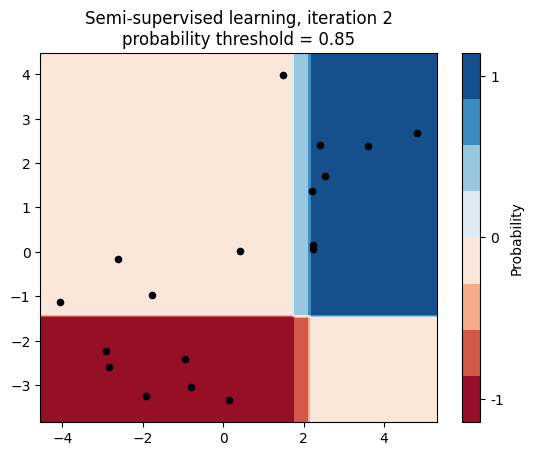
\includegraphics[width=0.5\textwidth]{images/img7.png}
    \caption{Wrapper Method Iteration 3}
    \label{fig:img7}
\end{figure}

\begin{figure}[H]
    \centering
    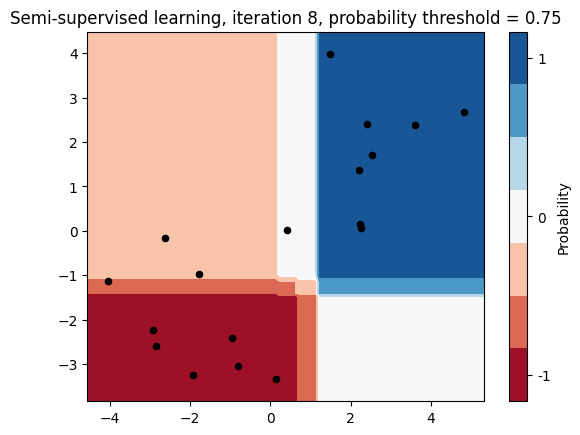
\includegraphics[width=0.5\textwidth]{images/img8.png}
    \caption{Wrapper Method Iteration 4}
    \label{fig:img8}
\end{figure}

\begin{figure}[H]
    \centering
    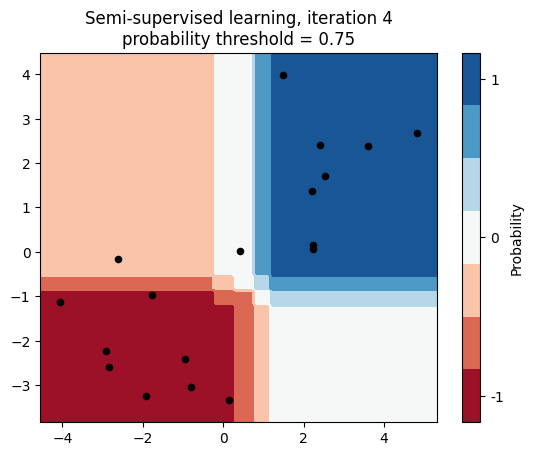
\includegraphics[width=0.5\textwidth]{images/img9.png}
    \caption{Wrapper Method Iteration 5}
    \label{fig:img9}
\end{figure}

\begin{figure}[H]
    \centering
    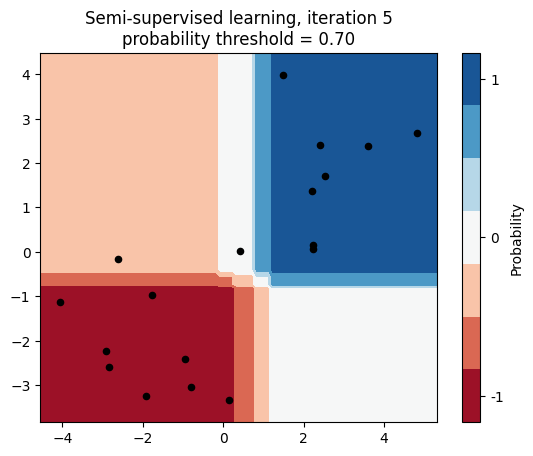
\includegraphics[width=0.5\textwidth]{images/img10.png}
    \caption{Wrapper Method Iteration 6}
    \label{fig:img10}
\end{figure}

\begin{figure}[H]
    \centering
    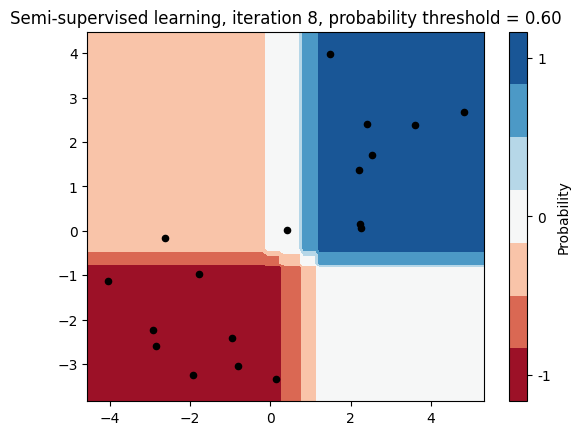
\includegraphics[width=0.5\textwidth]{images/img11.png}
    \caption{Wrapper Method Iteration 7}
    \label{fig:img11}
\end{figure}

\begin{figure}[H]
    \centering
    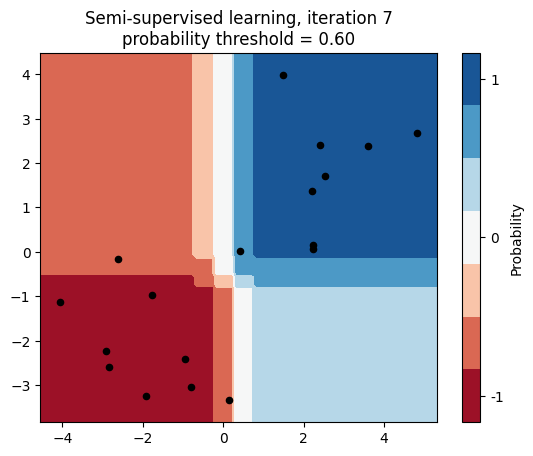
\includegraphics[width=0.5\textwidth]{images/img12.png}
    \caption{Wrapper Method Iteration 8}
    \label{fig:img12}
\end{figure}


Reviewing the iteration progress for the wrapper method provides an opportunity to inspect the results of the semi-supervised learning method. These graphs also have an attached colorbar on the right side of the figure. The colorbar ranges from -1 to 1 where -1 is class 1 and 1 is class 2. The colorbar is centered at 0, which is the unlabeled class.\par
This results of this method provided good results when the labeled data was near other members of the same class. However, the results were not good when the labeled data point was far away from its class members. I am unsure if this is a limitation of this method or if there is a bug in the implementation.

Finally, the assignment requests that all methods are plotted in the same figure. This is shown in figure~\ref{fig:img13}.

\end{multicols}

\begin{figure}[H]
    \centering
    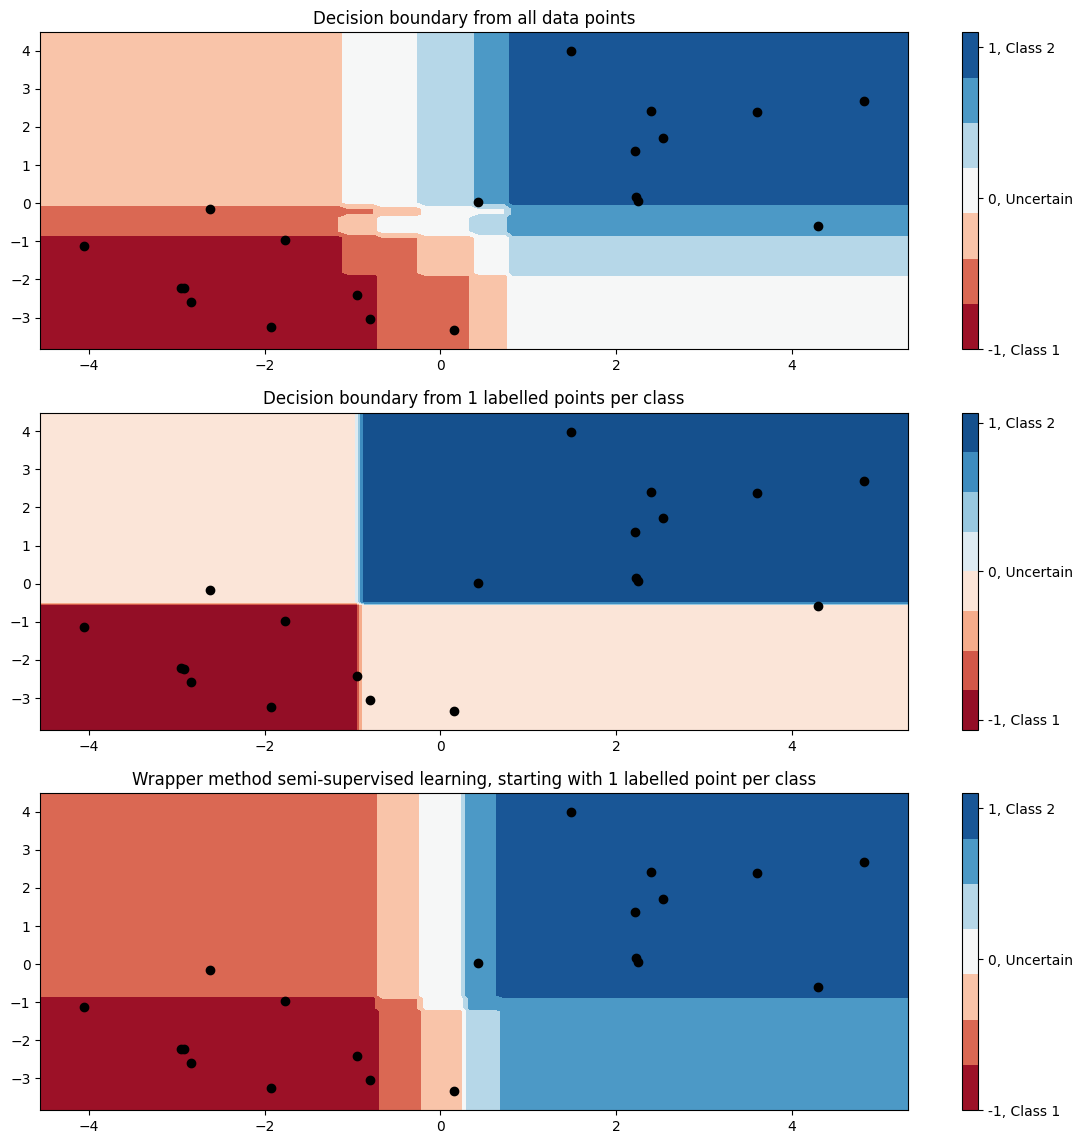
\includegraphics[width=0.9\textwidth]{images/img13.png}
    \caption{All Methods Plotted Together}
    \label{fig:img13}
\end{figure}

\begin{multicols}{2}



